
\documentclass[twoside]{article}
\setlength{\oddsidemargin}{0.25 in}
\setlength{\evensidemargin}{0.25 in}
\setlength{\topmargin}{-0.6 in}
\setlength{\textwidth}{6.5 in}
\setlength{\textheight}{8.5 in}
\setlength{\headsep}{0.75 in}
\setlength{\parindent}{0 in}
\setlength{\parskip}{0.1 in}


%
% ADD PACKAGES here:
%

\usepackage{amsmath,amsfonts,graphicx,amsthm,amssymb,thmtools}
\usepackage{hyperref}
\usepackage[ruled,vlined]{algorithm2e}
\usepackage{cancel}
\usepackage{multicol}
\usepackage{float}
\usepackage{subcaption}

\hypersetup{
    colorlinks=true,
    linkcolor=blue,
    filecolor=magenta,
    urlcolor=blue,
}

%
% The following macro is used to generate the header.
%
\newcommand{\customheader}[3]{
   \pagestyle{myheadings}
   \thispagestyle{plain}
   \newpage
   \setcounter{page}{1}
   \noindent
   \begin{center}
   \framebox{
      \vbox{\vspace{2mm}
    \hbox to 6.28in { {\bf EE 381V: Special Topics on Unsupervised Learning
        \hfill Spring 2018} }
       \vspace{6mm}
       \hbox to 6.28in { {\Large \hfill #1  \hfill} }
       \vspace{6mm}
       \hbox to 6.28in { {\it Professor: #2 \hfill Students: #3} }
      \vspace{2mm}}
   }
   \end{center}
   \vspace*{4mm}
}

%
% Convention for citations is authors' initials followed by the year.
% For example, to cite a paper by Leighton and Maggs you would type
% \cite{LM89}, and to cite a paper by Strassen you would type \cite{S69}.
% (To avoid bibliography problems, for now we redefine the \cite command.)
% Also commands that create a suitable format for the reference list.
%\renewcommand{\cite}[1]{[#1]}
%\def\beginrefs{\begin{list}%
        %{[\arabic{equation}]}{\usecounter{equation}
         %\setlength{\leftmargin}{2.0truecm}\setlength{\labelsep}{0.4truecm}%
%         \setlength{\labelwidth}{1.6truecm}}}
%\def\endrefs{\end{list}}
%\def\bibentry#1{\item[\hbox{[#1]}]}

%Use this command for a figure; it puts a figure in wherever you want it.
%usage: \fig{NUMBER}{SPACE-IN-INCHES}{CAPTION}
\newcommand{\indep}{\rotatebox[origin=c]{90}{$\models$}}
\newcommand{\fig}[3]{
			\vspace{#2}
			\begin{center}
			Figure \thelecnum.#1:~#3
			\end{center}
	}
% Use these for theorems, lemmas, proofs, etc.
\theoremstyle{definition}
\newtheorem{theorem}{Theorem}
\newtheorem{example}[theorem]{Example}
\newtheorem{lemma}[theorem]{Lemma}
\newtheorem{proposition}[theorem]{Proposition}
\newtheorem{claim}[theorem]{Claim}
\newtheorem{corollary}[theorem]{Corollary}
\newtheorem{note}[theorem]{Note}
\newtheorem{definition}[theorem]{Definition}
% \newtheorem{problem}{Problem}

% **** IF YOU WANT TO DEFINE ADDITIONAL MACROS FOR YOURSELF, PUT THEM HERE:

\declaretheoremstyle[%
headpunct={\medskip}, postheadspace=\newline, notebraces = {\quad}{},spaceabove = 8pt,spacebelow = 8pt]%
{problem}
\declaretheorem[name=Problem,style=problem]{problem}
\newcommand{\norm}[2]{\left\lVert #1 \right\rVert_{#2}}

%*****--------------------------------------------------------------------

\begin{document}
%\lecture{**Document-Title**}{**DATE**}{**Professor**}{**Students**}
\customheader{Improving Robust Manifold Defense}{Alex Dimakis}{Kwon Jeongyeol, Dany Haddad, Justin Lewis}

\newpage

\section{Introduction}
The success of adversarial attacks has brought increased scrutiny regarding the robustness of neural networks. A variety of defense methods have been proposed, and some of the more successful techniques are closely  related to the Invert and Classify (INC) approach \cite{ilyas2017}. INC uses a well-trained generative model to project a potentially adversarial image onto the manifold of natural images. This sister-image can now be safely classified as it no longer contains adversarial components which are far from the manifold. This process is not directly differentiable and therefore seemingly difficult to attack.

In response, our proposal was the following. Given the well-trained generator used for the Manifold Defense, train a matching encoder. Together, the generator and encoder form an autoencoder framework which is now directly differentiable and susceptible to adversarial attack. Although this framework could not be used to find adversarial examples; along the way, we discovered several useful results and robustness properties of the matched encoder. 

\subsection{Contributions}
Our contributions can be summarized as follows (listed in order of importance):
\begin{itemize}
    \item We introduce and formulate the training of a matched encoder to improve the INC defense.
    \item We critique the projection method used in the INC defense and give intuition for its instability. 
    \item We provide empirical evidence supporting the robustness of GAN-based defense methods.
\end{itemize}

\section{Background}
The following subsections will introduce basic notation for deep learning frameworks.
Additionally the notion of adversarial attack and training will be made clear. 

\subsection{Notation}

Dataset: $\{\mathcal{X},\mathcal{Y}\}$, a set of images $\mathcal{X}$ and corresponding
class labels $\mathcal{Y}$


Classifier: $\mathcal{C}_{\theta}$ 

GAN: generator $\mathcal{G}_{\phi}$ and discriminator $\mathcal{D}_{\psi}$

Autoencoder: encoder $\mathcal{E}_{\alpha}$ and decoder $D_\beta$

$x$: a natural image

$x_{adv}$: an adversarial image

\iffalse

\begin{multicols}{3}
%Column 1
Classifier: $\mathcal{C}_{\theta}$ 
\columnbreak
%Column 2
GAN: generator $\mathcal{G}_{\phi}$ and discriminator $\mathcal{D}_{\psi}$
\columnbreak
%Column 3
AE: encoder $\mathcal{E}_{\alpha}$ and decoder $D_\beta$
\end{multicols}


Given dataset $\{\mathcal{X},\mathcal{Y}\}$, a set of images $\mathcal{X}$ and corresponding
class labels $\mathcal{Y}$, a classifier $\mathcal{C}_{\theta}$ is tasked with correctly labeling the 
images in a held-out training set.

A Generative Adversarial Network with generator $\mathcal{G}_{\phi}$ and discriminator $\mathcal{D}_{\psi}$, 
is tasked with learning the underlying structure of $\mathcal{X}$ in an unsupervised fashion. 
\fi

\subsection{Adversarial Attacks and Training}
The notion of adversarial attacks is a phenomenon brought to light in the context of deep learning by Goodfellow et al. \cite{2014arXiv1412.6572G}. Within this work, it is argued that deep learning classifiers are less robust than previously assumed and susceptible to attack from an adversarial user. More specifically, given image $x$ with correct label $y$ (e.g. "cat") one can add a small perturbation $\delta$ to obtain a new image $x_{adv} = x + \delta$ which is now classified to the wrong label $y_{adv}$ (e.g. "peanut"). This adversarial example is crafted by using knowledge of the classifier $\mathcal{C_{\theta}}$ to maximize the difference between the true label $y$ and adversarial label $y_{adv}$. Given a appropriate notion of loss $L(y_{adv},y;\theta)$, a canonical adversarial attack is then conducted as follows:

\begin{problem}[Finding an adversarial example]
    \begin{equation*}
    \begin{aligned}
    & \underset{\delta}{\text{maximize}}
    & & L(y_{adv}(\delta),y;\theta) \\
    &
    & & y_{adv}(\delta) = \mathcal{C}_{\theta}(x + \delta) \\
    & \text{subject to}
    & & \norm{\delta}{p} \leq \epsilon
    \end{aligned}
    \end{equation*}
\end{problem}

Plainly said, find the adversarial image $x_{adv} = x + \delta$ within an $\epsilon$ sized $\ell_p$ ball around the
original image which fools the classifier the most. Commonly, this optimization problem is approximately solved using
one of two approaches: Fast Gradient Sign Method (FGSM) and projected gradient descent (PGD). It has been empirically
verified that FGSM attacks are less effective at fooling a classifier than PGD approaches \cite{madry}. Note, a suitable
loss function $L(x,y;\theta)$ might be cross-entropy loss for multi-label classification. 


\begin{figure}[H]
    \caption{diagrams demonstrating FGSM (left) and PGD (right) given $\delta$ within an $\ell_2$ ball}
    \centering
    \begin{tabular}{ccc}
    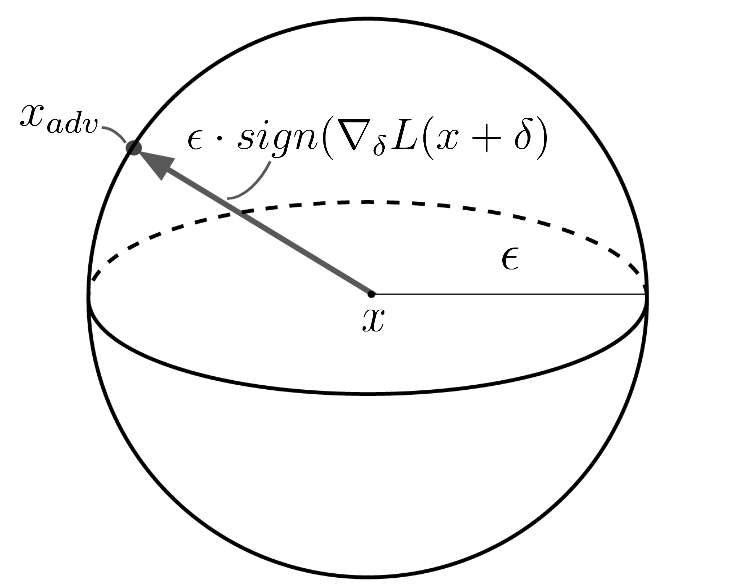
\includegraphics[scale=0.2]{./FGSM.png}
    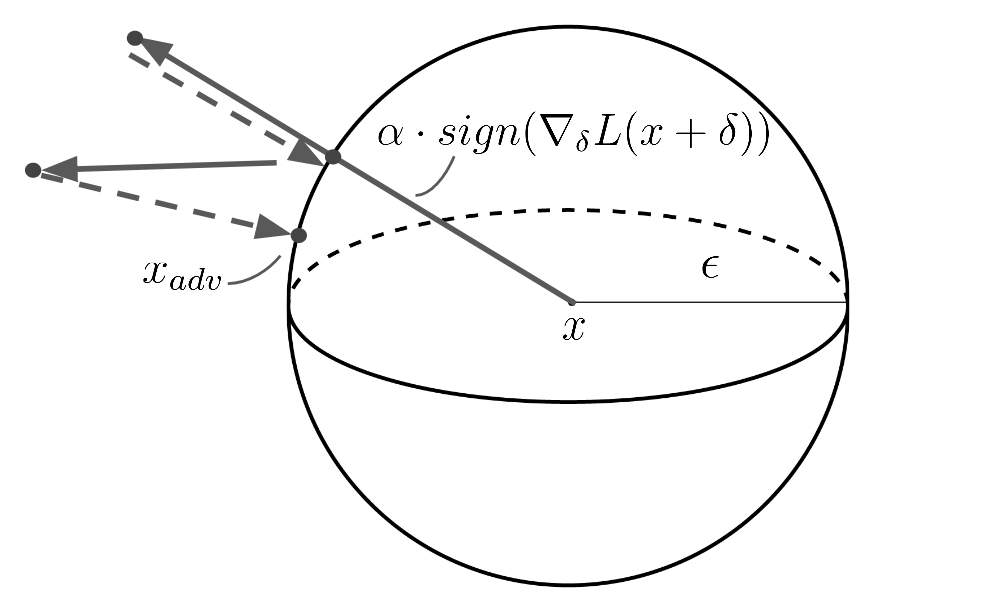
\includegraphics[scale=0.2]{./PGD.png}
    \end{tabular}
    \label{fig:my_label}
\end{figure}

%There are a number of different environment assumptions that can be made to result in different attack models.
%The above attack is a white-box, non-targeted attack.

In order to defend against adversarial attacks, a number of defense strategies have been employed \cite{athalye2018}.
The most straightforward defense strategies introduce adversarial examples $\mathcal{X}_{adv}$ into the set of training images
$\mathcal{X}$, which allows the network to learn to correctly classify even these examples. Other methods try to 
"detect" adversarial examples. Essentially, these defense strategies give no clear guarantees and the process of
attack-defend becomes an arms-race. 

\section{Invert and Classify Defense}
The defense strategy of particular interest to our work is the Invert and Classify (INC) approach as introduced by \cite{ilyas2017} and a very similar technique developed by \cite{pixel}. As mentioned before, INC leverages the strong representation power
of GANs. The idea is to project an adversarial image onto the range of a GAN and classify this 'cleaned' image.
This is done using gradient descent. If the GAN approximates the manifold of natural images well enough, and
the gradient method projects onto the manifold well enough, then the INC strategy is feasible.

\begin{figure}[H]
    \caption{abstract diagram demonstrating the inversion portion of INC}
    \centering
    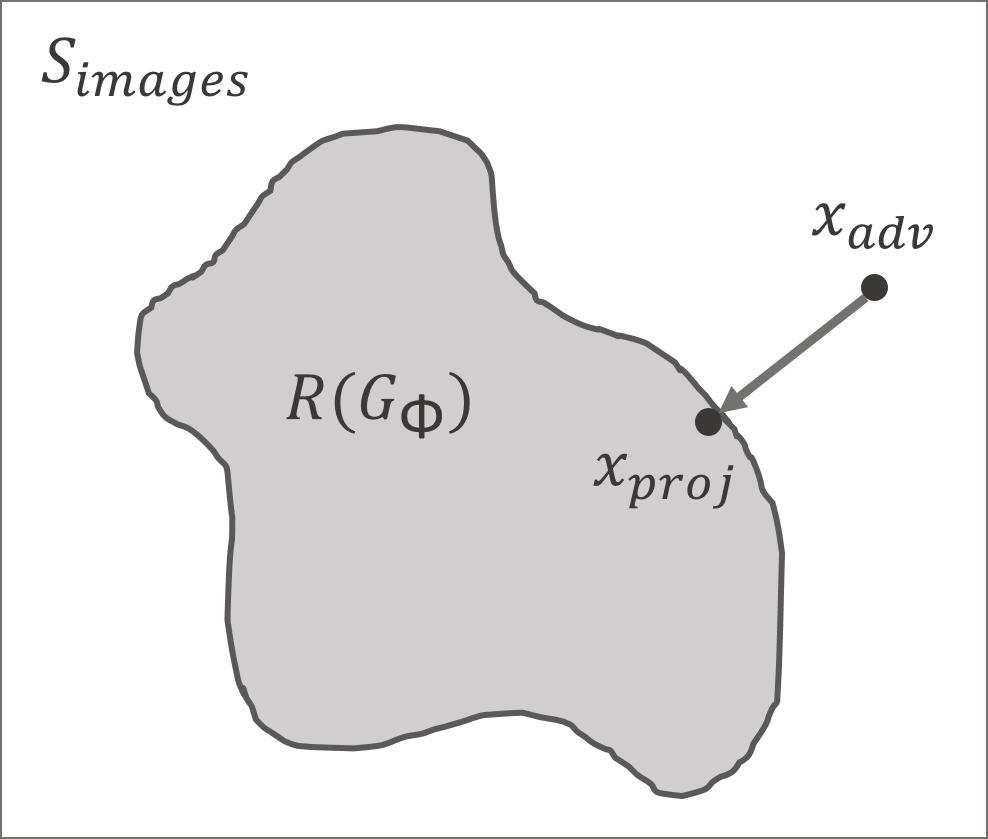
\includegraphics[scale=0.3]{./projection_diagram.png}
    
    $S_{images}:$ the space of all images 
    
    $R(G_{\phi}):$ the range of the generator
    \label{fig:my_label}
\end{figure}

In order to project onto the range of the GAN, the optimization defined in Problem 2 is approximately solved by gradient descent. The descent steps search through the latent space $\mathcal{Z}$ for an optimal value $z^*$ which provides the projection $x_{proj} = G_{\phi}(z^*)$. This projection is visually similar to $x_{adv}$ in terms of the $\ell_\infty$ norm. It should be noted that without a trained encoder, the inversion step must begin with a random initialization. It was found empirically in \cite{ilyas2017} that with random initialization, the INC method had poor stability at the output. Therefore, many random initializations were necessary, and the best result was used as the final projection. This repetition of the inversion step is very costly, as it can take thousands of gradient steps per iteration. The high computation cost of the INC defense is a fairly large drawback. In section 5 we elaborate on this and provide a solution to this problem. In figure 3 below, the entire INC process is summarized graphically. 

\begin{figure}[H]
    \caption{the INC defense method}
    \centering
    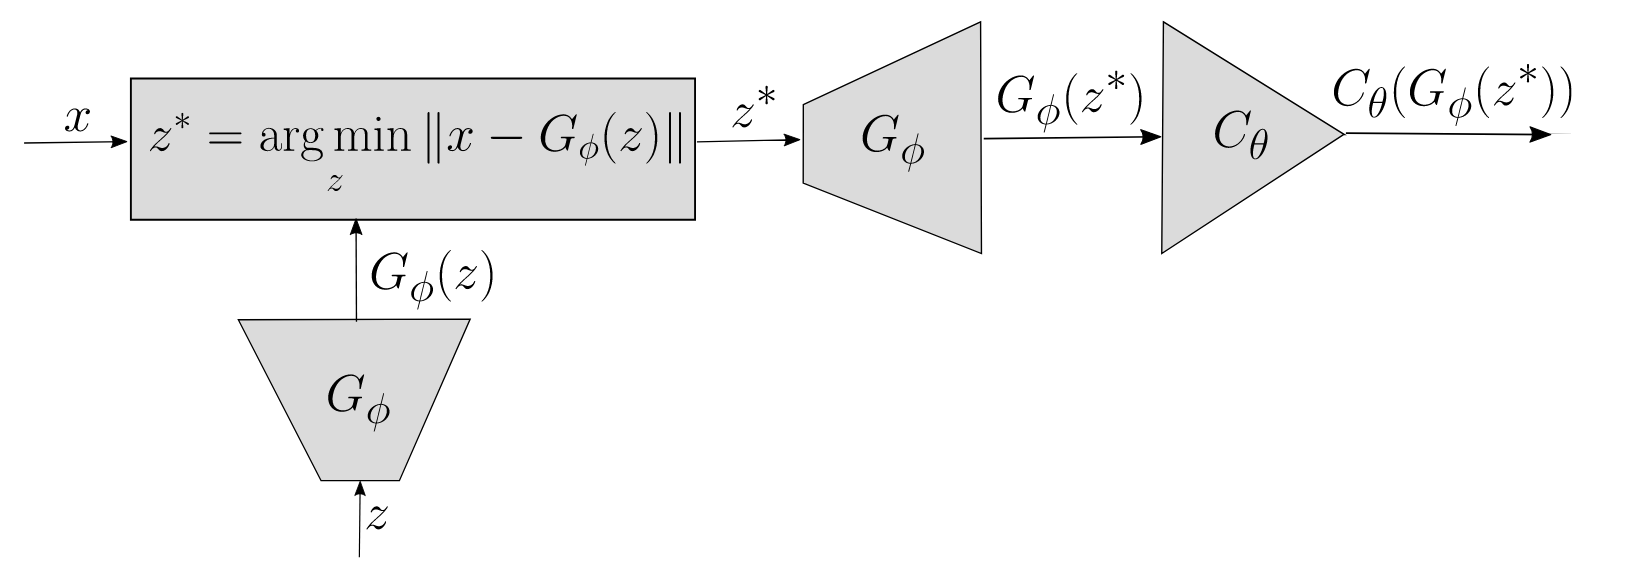
\includegraphics[scale=0.25]{./INC_diagram.png}
\end{figure}

\begin{problem}[INC projection step (in $\mathcal{Z}$ space)]
    \begin{equation*}
    \begin{aligned}
    & z^* = \text{arg } \underset{z}{\text{min}}
    & & \norm{\mathcal{G}_{\phi}(z)-x_{adv}}{2}^2 \\
    \end{aligned}
    \end{equation*}
\end{problem}


\newpage

\section{Adversarial Attack on INC}
Similar to the Backward Pass Differentiable Approximation (BPDA) method of Athalye et al., we propose to attack the INC defense mechanism by building a differentiable approximation for the process of projecting onto the manifold of natural images. Using this approximation, we can approximately evaluate the gradient $\nabla_{\delta} L(y_{adv},y) $ and perform gradient based attacks (FGSM and PGD). We learn this approximation by training an encoder  $\mathcal{E}_{\alpha}$ that performs the inverse operation of the generative model used in the INC process. In this way, passing an image through the encoder and pre-trained generator will give us the reconstruction $\hat{x} = \mathcal{G}(\mathcal{E}_{\alpha}(x_{adv}))$. This image serves as an approximation to the result of the INC projection process, $x_{proj}$. To learn this encoder, we approximately solve the following problem by SGD:

\begin{problem}[Learning a matching encoder $\mathcal{E}_{\alpha}$]
    \begin{equation*}
    \begin{aligned}
    & \underset{\alpha}{\text{minimize}}
    & & \mathbb{E}_{Z} [||\mathcal{E}_{\alpha}(\mathcal{G}(Z)) - Z||_2^2]
    + \lambda \cdot \mathbb{E}_{X} [||\mathcal{G}(\mathcal{E}_{\alpha}(X)) - X||_2^2]\\
    \end{aligned}
    \end{equation*}
\end{problem}

The loss function given in Problem 3 can be interpreted as a sum of two reconstruction loss terms. The first in the latent space $\mathcal{Z}$ and the second in the image space $\mathcal{X}$. Together, the reconstruction terms impose a form of cycle consistency between the image and latent spaces. We empirically found that training an encoder that perfectly matches the pre-trained generator $\mathcal{G}_{\phi}$ is difficult; however, the reconstruction formed by the composition of encoder and generator was good.

\begin{figure}[H]
    \caption{matched encoder + generator defence model}
\begin{center}
    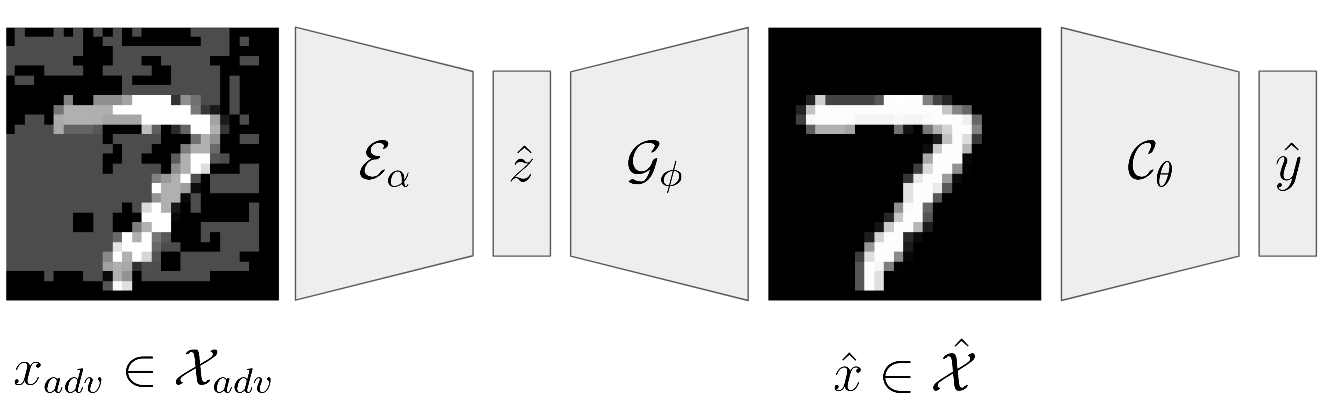
\includegraphics[scale=0.3]{./INC.png}
\end{center}
\end{figure}

With a trained encoder $\mathcal{E}_{\alpha}$ and pre-trained generator $\mathcal{G}_{\phi}$ pair, one can now attempt to attack the INC defense by differentiating through the entire classification pipeline. This three-part model is detailed in figure 4. The caveat of our approach is that the trained encoder must sufficiently approximate the projection step from the INC defense, i.e. $\mathcal{E}(x_{adv}) \approx z^*$. To find an adversarial example, we turn to FGSM or PGD to approximately solve the same formulation from Problem 1 with a modified loss which is now parameterized by all three networks. We empirically found that this direct approach was not very effective (the classification accuracy remained at 93 \% ). 

\begin{problem}[Direct adversarial attack on INC]
    \begin{equation*}
    \begin{aligned}
    & \underset{\delta}{\text{maximize}}
    & & L(x+\delta,y;\{\alpha,\phi,\theta\}) \\
    & \text{subject to}
    & & \norm{\delta}{p} \leq \epsilon
    \end{aligned}
    \end{equation*}
\end{problem}

Stepping back, we decided to then attack the INC defense indirectly. With a trained encoder, we could then add adversarial noise to push the encoding $\mathcal{E}(x_{adv})$ as far away from the "true" encoding $\mathcal{E}(x)$ as possible (within the limits of an $\epsilon$ bounded attack).

\begin{problem}[Indirect adversarial attack on INC]
\begin{equation*}
\begin{aligned}
& \underset{\delta}{\text{maximize}}
& & \norm{\mathcal{E}(x+\delta)-\mathcal{E}(x)}{2}^2 \\
& \text{subject to}
& & \norm{\delta}{p} \leq \epsilon
\end{aligned}
\end{equation*}
\end{problem}

%The intuition behind this indirect attack is that the encoding of two images with the same class or form are likely to be close in the latent space $\mathcal{Z}$.
By pushing the encoding $\mathcal{E}(x_{adv})$ far away, this attack hopes to cause the INC projection step to diverge to the wrong class. This is reasonable so long as the encoder adequately approximates the INC projection step. In the end, we empirically found that this indirect attack was unable to find "true" adversarial images. Rather, the results generated from the optimization of Problem 4 were $x_{adv}$'s which reside at the boundary of two classes. These sort of images are ones which have no obvious class, and therefore not adversarial in the usual sense. 

(include examples of adversarial images?)

\section{Encoder Improvement on INC}
Although training a matching encoder and then attacking the INC defence was ineffectual, we did find an interesting phenomenon. We empirically discovered that $\Hat{z} =\mathcal{E}_{\alpha}(x_{adv})$ provided a very good initial point for the INC projection step. With a much better initialization, the number of gradient steps needed to converge was reduced significantly from one thousand to several hundred (for the same level of reconstruction quality). Additionally, this method of encoding for good initialization resulted in higher classification robustness. This is attributed to the instability of using gradient descent for projection. Even if many random initializations are used, the INC projection may not converge to an image of the correct class. By using the encoder as an initial point, the probability of correct convergence is increased (for a fixed number of projection steps). 

\begin{figure}[H]
\centering
\caption{Random vs. encoded initialization for random MNIST images (150 projection steps each)}
\begin{tabular}{ccc}
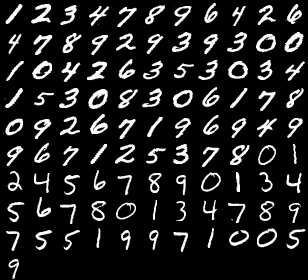
\includegraphics[width=2in]{reconstr_original.png} &
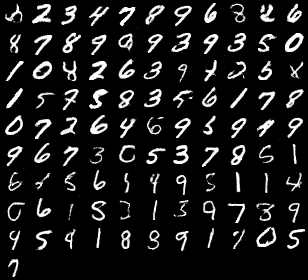
\includegraphics[width=2in]{reconstr_random_z.png} &
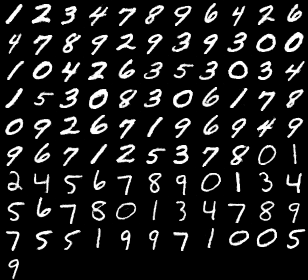
\includegraphics[width=2in]{reconstr_encoded.png} \\
random MNIST images (left) &
$x_{proj}$ from random z (center) & 
$x_{proj}$ from $\hat{z} = \mathcal{E}_{\aplha}(x)$ (right)
\end{tabular}
\end{figure}

As shown in figure 5, the reconstruction formed by using the initial point $\hat{z} = \mathcal{E}_{\aplha}(x) $ is visually superior; moreover, the image class is preserved with higher probability. Note that these examples are not adversarial which highlights the issue of using a random initialization. Our improved INC defence model is detailed graphically in figure 6. 

\begin{figure}[H]
\centering
\caption{INC + matched encoder defense method }
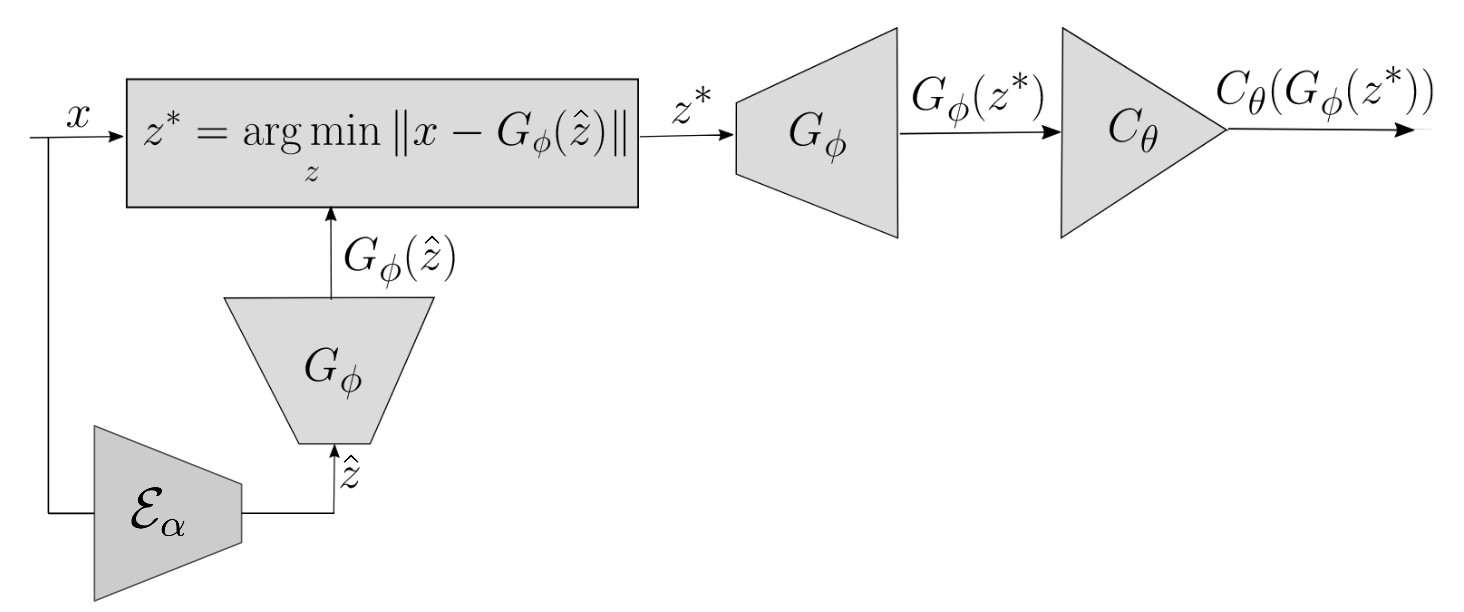
\includegraphics[scale=0.25]{INC++.png}
\end{figure}

(need reconstruction difference examples for adversarial images, similar to figure 5)

\section{Critique of INC Projection}
We empirically found that using a matched encoder for initialization added robustness; moreover, it is interesting to consider why projection with random initialization is generally unstable. The two claims that follow attempt to explain intuitively why this is.

\subsection{Projection with Image Space Loss}
Looking back to the INC projection step from Problem 2, at first the formulation seems innocuous. We hope to find a $z^*$ which results in projection $x_{proj} = \mathcal{G}_{\phi}(z)$ which is close to $x_{adv}$.

\begin{equation*}
\begin{aligned}
& z^* = \text{arg } \underset{z}{\text{min}}
& & \norm{\mathcal{G}_{\phi}(z)-x_{adv}}{2}^2 \\
\end{aligned}
\end{equation*}

The problem with this formulation is that the loss is defined as an $\ell_2$ distance in the image space. Our claim is that this loss surface in the z-space is ill-conditioned with many sharp minima. For a given image class, there are a large number of candidate images (not necessarily of the same class) which produce a small $\ell_2$ loss with the true image. Assuming random initialization, we believe the INC projection is likely to fall into one of these sharp valleys and not escape.

In order to make this idea more concrete, we consider a simple example. Let us assume that our data comes from a Swiss roll distribution. Given a test example we wish to classify, $x$ (corresponding to location \emph{D} in the figure below), we wish to find $z$ such that $||G(z) - x||_2$ is small. Say that the random initialization point we choose corresponds to location \emph{A} in the figure below. Using gradient descent, the projection process will encounter several local minima before reaching the optimal point $z^*$ which gives us the smallest reconstruction error.

\begin{figure}
\begin{subfigure}{0.5\textwidth}
    \caption{Swiss roll data in $\mathbb{R}^2$}
    \centering
    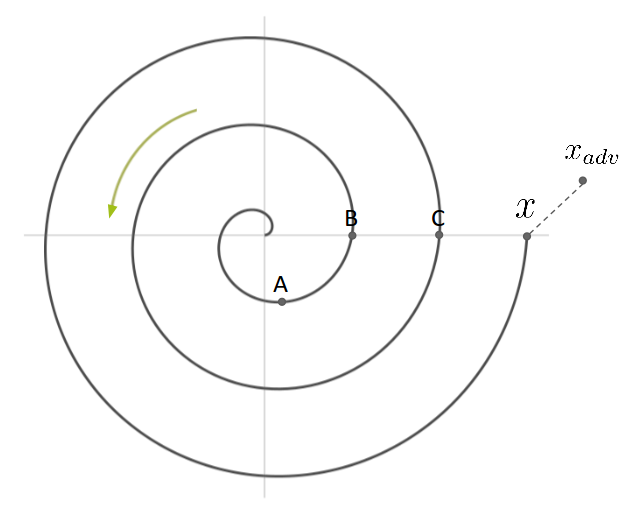
\includegraphics[scale=0.25]{./swiss.png}
\end{subfigure}%
\begin{subfigure}{0.5\textwidth}  %%<--- here
    \caption{Data loss vs z $\mathbb{R}^2$}
    \centering
    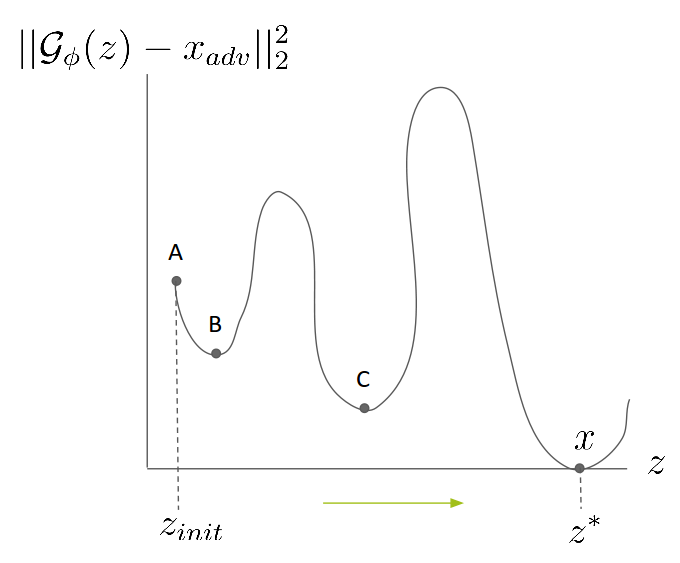
\includegraphics[scale=0.25]{./loss_swiss.png}
\end{subfigure}
\end{figure}

.... (include example from Kwon's intial experiments)

\subsection{Random Initialization}

In addition to an ill-conditioned loss surface, the INC projection step encounters another problem, now due to the random initialization. Our second claim is that for high dimensional latent spaces, the random encoding $z_{init}$, used as the starting point for optimization, is likely far from the true encoding $z$.

\begin{figure}[H]
    \caption{Most of the probability mass is contained in a shell of width $\frac{1}{d}$ where $d$ is the dimension}
    \centering
    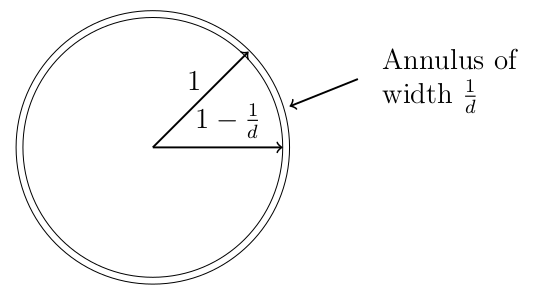
\includegraphics[scale=0.3]{./shell.png}
\end{figure}

For Gaussian ($N(0, 1)$) random vectors in high dimensions, $||u - v||_2^2 \approx O(d)$ \cite{foundations}, so a random initialization point in the latent space is far from the optimal $z^*$ w.h.p. Accordingly, it is very likely that we will fall into a local minimum during the projection step of INC.

The true encoding $z$ and initialization $z_{init}$, both drawn from $\mathcal{N}(0,\sigma^2 \cdot I) \in \mathbb{R}^N$, are independent; thus, we can simply use the LLN to state:

$\norm{z-z_{init}}{2}^2 = \sum\limits_{i=1}^N (z_i-z_{init,i})^2 \overset{p}{\longrightarrow} N \cdot \mathbb{E}[(Z-Z_{init})^2]
= 2N \cdot \mathbb{E}[Z^2] = 2N \cdot \sigma^2$


(need example images showing the reconstruction created by using encoder + generator)

\section{Classification Experiments}

Our classification experiments were conducted on the familiar MNIST dataset. The adversarial images $\mathcal{X}_{adv}$ were generated through FGSM attacks on the unprotected classifier $\mathcal{C}_{\theta}$. The classification accuracy results
are presented below.

\begin{itemize}
    \item Clean test data: 98\%
    \item Adversarial test set using FGSM against unprotected classifier and $\epsilon = 0.2$: 19\%
    \item Adversarial test set against INC protected classifier: 87\%
\end{itemize}

(maybe add some diagrams of adversarial examples here?)

\section{Future Work}

\section{Conclusion}

%*****--------------------------------------------------------------------
\bibliographystyle{plain}
\bibliography{ref}

\section{Appendix}

\subsection{Direct Attack on INC}

Using our BPDA style attack on an INC protected classifier (differentiating through an encoder fitted to the generator used in the INC process) we did not arrive at the results that we had hoped for: the accuracy of the INC protected classifier remained at 93\%. Shown below are the original images, the adversarial examples created via FGSM and the images resulting from the autoencoding process.

\begin{figure}[H]
\centering
\begin{tabular}{ccc}
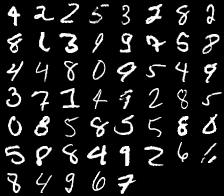
\includegraphics[width=2in]{cl_original.png} &
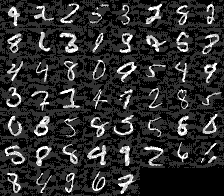
\includegraphics[width=2in]{cl_adversarial.png} &
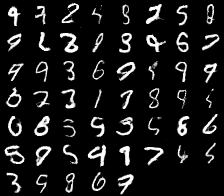
\includegraphics[width=2in]{cl_reconstr.png}
\end{tabular}
\caption{Some failure cases in MNIST test data, the adversarial examples created via FGSM and the images resulting from the autoencoding process}
\end{figure}

\end{document}